\documentclass[a4paper,11pt, usenatbib]{article}
% a4paper sets it up with the measures for A4 paper
% 12pt is the lettering size, (you can use 11pt or 12pt)
\usepackage[sort, numbers]{natbib}
\bibliographystyle{IEEEtran.bst}
% this produces A4 pages with a lot more text on each page
\usepackage{a4wide}
\usepackage[utf8]{inputenc}
\usepackage{fullpage}
\usepackage{amsmath}

%\bibliographystyle{natbib}

\usepackage{graphicx}
\usepackage{wrapfig}
\usepackage{amssymb}
\usepackage[]{algorithm2e}
%useful for dealing with labels, uncomment while writing
%\usepackage{showkeys}


% if you prefer the equations numbered consecutively comment out
% the following line AND all the
% \setcounter{equation}{0} after every \section command
\renewcommand{\theequation}{\thesection.\arabic{equation}}

\begin{document}

%%%%%%%%%%%%%%%%%%%%%%%%%%%%%%%%%%%%%%%%%%%%%%%%%%%%%%%%%%%%%%%%%%%%%%%%%%%
% first as you might guess the title page
\begin{titlepage}
% flushright puts it towards the right of the page
\begin{flushright}
% our preprint number yy-nn (year-number), ask your supervisor how to get this
LU TP 14-nn\\
% some indication of the date
June 2019\\
\end{flushright}
\vfill
\begin{center}
% put in line breaks to make the title look nicer and provide more
% space between the lines
{\large\bf Improving the Generalization of the Sibling-Descendant Cascade-Correlation Learning Architecture}
\\[3cm]
{\bf John Ringdahl}
\\[5mm]
{Department of Astronomy and Theoretical Physics, Lund University}
\\[2cm]
{Bachelor thesis supervised by Patrik Edén}
\vfill
% use the eps version for latex and the pdf version for pdflatex 

\includegraphics[height=4cm]{logocLUeng.png}
%
\includegraphics[height=4cm]{logocLUeng.pdf}
\end{center}
\end{titlepage}
%%%%%%%%%%%%%%%%%%%%%%%%%%%%%%%%%%%%%%%%%%%%%%%%%%%%%%%%%%%%%%%%%%%%%%%%%%%
% a page with the abstract and popular description
\thispagestyle{empty} % do not count pages just yet

% these 'rubber' spaces make the page layout look nicer
%the \phantom{p} is to make something there for the \vfill to push against
\phantom{p}
\vfill

\section*{Abstract}


\vfill
\newpage
\section*{Artificiella Hjärnor till Alla}
% Swedish letters: \"a, \"o, \aa or ä, ö, å if you use utf8
 \begin{wrapfigure}[13]{r}{0.4 \textwidth}
 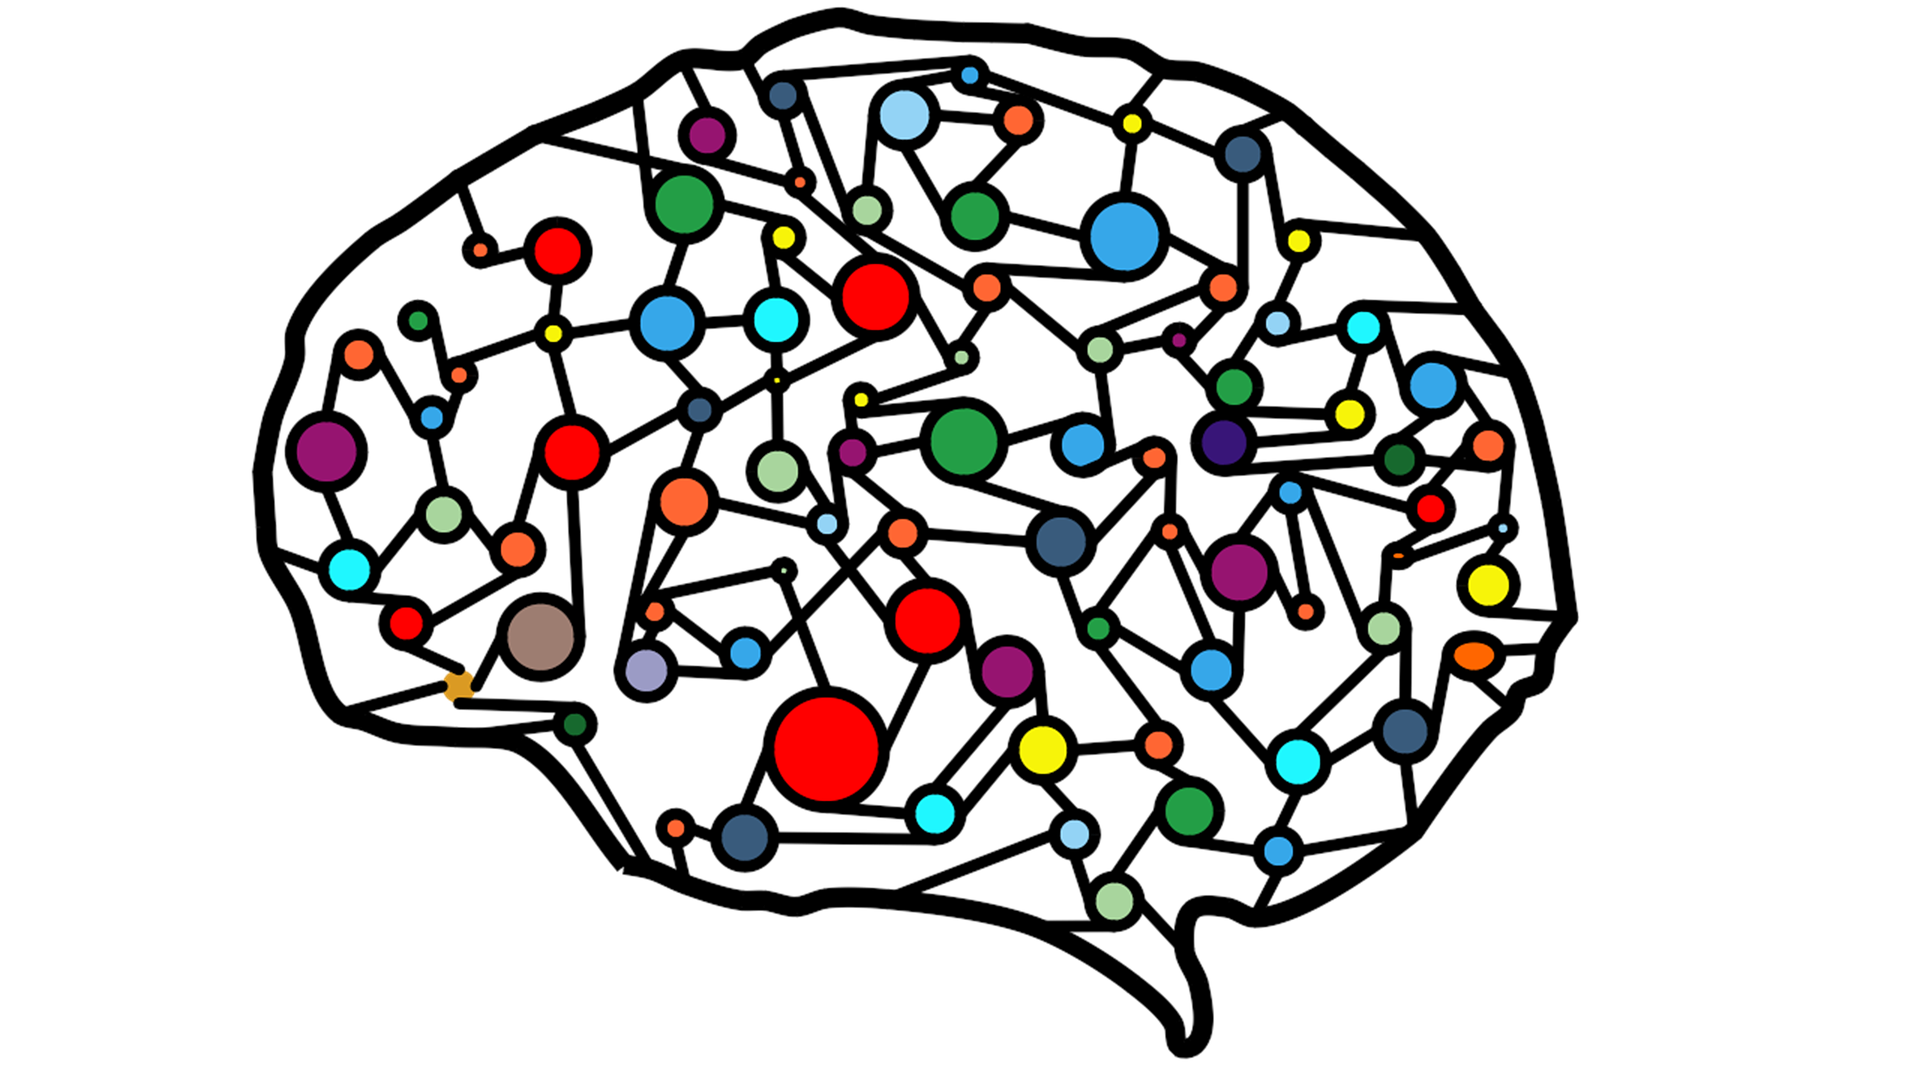
\includegraphics[width=0.38 \textwidth, trim={9cm, 0, 10cm, 0}, clip]{artificial-neural-network-3501528_1920}
 \end{wrapfigure}
 
 %What if Apple’s Siri could fill in a form for you at work? Or if you could have your Google Assistant plan your grocery shopping for the week? What if all mundane tasks that you do routinely without deeper thought were handled automatically by an AI? Entertaining as this scenario might be, the future where everyone has a universal virtual assistant is still far off. However, while a universal AI is difficult to make, it is a lot easier to make AIs that are specially designed for a single task. In other words, we might soon all have access to a personal workforce of specialized virtual assistants that can relieve us from mundane tasks so that we have more time for activities we enjoy. 
 
Tänk om Apples Siri kunde fylla i en blankett åt dig på jobbet. Eller om Google Assistant planerade veckans inköpslista. Tänk om alla banala sysslor som du utför rutinmässigt utan någon djupare åtanke kunde skötas automatiskt av en artificiell intelligens, AI. Hur underhållande detta scenarie än får vara så är en framtid där alla har en personlig universall assistent fortfarande långt borta. Men även om en universall AI är svår att skapa så är det relativt enkelt att skapa AI som är specialiserade på enskilda uppgifter.  Med andra ord, vi har kanske snart tillgång till en personlig arbetsstyrka av specialiserade virtuella assistenter som kan underlätta alla banala sysslor så att vi har mer tid för aktiviterer som vi gillar. 
 
%A basic AI is made up of what is called an artificial neural network, or ANN for short. An ANN is like a digital brain with digital neurons connected to each other with digital axons. And like a human brain, an ANN can process information and come up with a conclusion. For example, trying to predict the weather in an hour based on the current weather. Similar to a baby, an ANN is born clueless. It does not know that a cat is a cat unless it is told, and then it might confuse a dog with a cat unless it is told the difference. For an ANN to be useful it first needs to learn by example. But contrary to humans, ANNs can learn things ‘too well’, so that they become too fixated on the examples and can’t apply what they have learned to new scenarios. An analogy would be if a person learned to understand British English, but then fails to understand American English due to the difference in pronunciation.

En enkel AI är uppbyggd av vad som kallas ett artificiellt neuron nätverk, eller ANN. Ett ANN liknar en digital hjärna med digitala neuroner som är ihopkopplade med digitala axoner. Och som en mänsklig hjärna kan den hantera information och komma med en slutsats. Det kan till exempel vara att försöka förutsäga vädret om en timme baserad på hur vädret är för tillfället. I likhet med en bebis föds en ANN helt ovetande om sin omvärld. Det vet inte att en katt är en katt om den inte blir tillsagd, och då kommer det kanske förväxla en hund med en katt om den inte blir \textbf{tillsagd} vad som är skillnaden. För att ANN ska vara användbara måste de lära sig genom exempel. Men till skillnad från en människa kan ANN lära sig 'för bra' genom att fixera sig för mycket på exemplen så att de inte kan använda det de har lärt sig på nya scenarier. En liknelse skulle vara om en människa skulle lära sig att förstå brittisk engelska men sen inte kunna förstå amerikansk engelska på grund av att de skiljer sig i utal.

%Returning to our idea of a workforce of AIs, the problem of creating such a workforce is that everyone has different needs. An AI that grades high-school English essays still needs to be highly complex to be able to handle essays on all topics and from all high schools. The best way would be to create an AI for each individual assignment. And there lies the heart of the problem; we are not yet able to mass produce AIs. As of now, most AIs need to be designed manually, and that requires both expertise and time. That means that task-specific AIs are limited to those who are willing to invest the money needed to produce them. Currently, this mostly applies to tech companies and medical researchers.

Om vi återvänder till idén om en arbetstyrka av AI så är problemet med att göra en sådan arbetstyrka är att alla har olika behov. En AI som betygsätter gymnasieuppsatser behöver fortfarande vara väldigt avancerad för att kunna hantera uppsatser om alla ämnen och från alla gymnasier. Det bästa lösningen skulle vara att ha en AI för varje uppgift. Det är där problemets kärna ligger, vi kan ännu inte massproducera AI. Än så länge så måste de flesta AI designas manuellt, och det kräver både expertis och tid. Vilket betyder att uppgiftsspecifika AI är begränsade till dem som är villiga att investera pengarna som behövs för att producera dem. För tillfället gäller det för det mesta för tech-företag och medicinsk forskning.

%One way to build ANNs for AIs without the need of carefully designing them is Cascade-Correlation Learning Algorithm, shortened to Cascor. Without going into too much detail, Cascor builds the ANN, adding neurons, as it learns, so that the structure adapts to the complexity of the problem at hand. The problem with Cascor is that the ANNs that are produced are easily fixated on the learning examples and will perform more poorly on the tasks they were designed for than traditional ANNs. 

\textit{The Cascade-Correlation Learning Algorithm}, eller \textit{Cascor}, \textbf{är ett sätt att bygga ANN utan att behöva noggrant designa dem.} Utan att gå in på för många detaljer så bygger Cascor ANN, genom att lägga till neuroner, medan den lär sig. Så strukturen anpassar sig efter problemet i fråga. \textbf{Problemet med Cascor är att nätverken som produceras väldigt lätt fixeras sig på träningsexemplerna och kommer då prestera sämre på uppgifterna som de var designade för jämfört med traditionellt designade nätverk.}

%The aim of this thesis is to explore ways of increasing the performance of ANNs constructed with Cascor. Hopefully, this will lead to new ways of producing adequate ANNs that are easy to use and make simple AIs more accessible to the public.

Målet med denna uppsats är att undersöka sätt som man kan förbättra ANN som är byggda med Cascor. Förhoppningsvis kommer det leda nya metoder för att producera funktionsdugliga nätverk som är lätta att använda och som gör simpla AIn mer tillgängliga för allmänheten.

\vfill

\newpage

\tableofcontents
% the list of figures and tables is optional
\listoffigures 
\listoftables


\newpage
\section{Introduction}
\setcounter{equation}{0}
\label{sec:introduction}


%\textbf{Introducing ANNs}

Artificial neural networks, ANNs or just neural networks, are fast becoming a key instrument in computer science and modern technology. The development during the last few decades has established neural networks as a powerful tool within data analysis within many fields of research as both a function approximator\cite{hornik_multilayer_1989} and a classifier\cite{zhang_neural_2000}. They are aiding researchers in tasks such as: medicinal diagnosis\cite{amato_artificial_2013}, time-series predictions\cite{zhang_investigation_2001}, and image recognition\cite{simonyan_very_2014}. \textbf{sentence transition, more? Commercial use?} 

%Their uses ranges from classification and regression in data analysis to ... .In research, ANNs have proven to be a powerful tool for data analysis and sequence predictions. This is most notable in biology and medicinal science, where neural networks are used to identify species\cite{alhady_butterfly_2018} or diagnose illnesses\cite{ahmed_artificial_2005}. 

%Machine learning is more relevant now than ever before. The advances in the field over the last decade, along with the increase in computer power, has made an impact in our everyday life in many forms. For example, virtual assistants have been in our phones for some time now, and they are using artificial neural networks, ANNs, to recognize speech, and modern autopilots in cars are able to avoid accidents by automatically braking or steering away\cite{noauthor_autopilot_nodate}. This is most notable in biology and medicinal science, where neural networks are used to identify species\cite{alhady_butterfly_2018} or diagnose illnesses\cite{ahmed_artificial_2005}.

%\textbf{Introducing CC}

The Cascade-Correlation learning architecture, Cascor, is a constructive learning algorithm for neural networks developed by Fahlman and Lebiere\cite{fahlman_cascade-correlation_1990}. It was originally designed to to be a faster alternative to the existing learning algorithms, most notably back-propagation, with the added benefit of constructing the networks during training. \textbf{Cascor accomplishes this by training the hidden nodes separately one at the time and freezing their input weights when they are added to the network.} This allow the nodes to focus on finding one feature at the time instead of having \textbf{all the nodes searching for all the features} simultaneously while trying to accommodating for each other, which is known as the moving target problem\cite{fahlman_cascade-correlation_1990} \textbf{more mentions}. The new nodes have input connections from every preceding layer, and thus the networks \textbf{created} have complete feed forward connections, including all shortcut connections. To decrease the probability of a poorly performing node being added to the network, a pool of nodes is trained. Then, the best node is chosen to be implemented into the network.

One early criticism of Cascor was that every added node forms a new layer, which results in a potentially excessive depth of the networks\cite{phatak_connectivity_1994}. Fahlman and Baluja responded to this criticism with an alternative method called Sibling/Descendant Cascade-Correlation, SDCC, that allowed for nodes to be added to the same layer as the last node \textbf{(currently deepest layer?)} as well as forming a new layer\cite{baluja_reducing_1994}. However, even though SDCC is able to substantially reduce the network depth without a large impact on the performance, there has not been much follow-up \textbf{work on the algorithm}. Most of the later research has been on the original Cascor algorithm or other modification of Cascor[\textit{sources}]. 

%\textbf{Flaws with ANNs (that can be solved with CC)}
%Back-propagation is the most common learning algorithm for neural networks. 

%Another problem with ANNs is that the networks need to be designed manually. The number of layers and how many nodes there are in each layer need to be decided before training begins, and each problem requires differently structured networks in order to function optimally. If a network is too big it is more easily overfitted, and if it is too small it won’t be able to solve the task. Often you need to do some trial-and-error in order to find a good architecture. This requires the training of multiple networks, which can be computationally demanding and slow.

%\textbf{Introducing CC and SDCC}

%The Cascade-Correlation learning architecture was designed to almost completely circumvent this problem of choosing an architecture . It builds the network during training; starting with just an input and output layer, and then adding hidden nodes that have been individually trained in order to reduce the error. This method also doubles as a feature detector: the hidden nodes are trained to find the most important feature of the data set that has not been discovered yet. The nodes that are added have their input weights fixed, and thus, only one layer of weights is trained at the time. This makes the algorithm less computationally demanding than conventional training.

%\textbf{Flaws with SDCC to try to solve}

\textbf{The networks built with Cascor can be prone to overfitting \cite{lahnajarvi_evaluation_2002, balazs_cascade-correlation_2009}. One reason for this could be that in Cascor are the weights are frozen when added to the network. Thus, there are no network wide adaptations during training and no cooperation between the nodes to find the optimal features of the data set. As such, the generalization is no longer only a property of the whole network, but also something to be considered with each node in the network. }

%\textbf{Aim and goal}

This thesis will use a validation set that is not used in the node training when choosing the nodes that are added to the network. The aim is to study how such a validation set can be used in order to improve the generalization of the produced networks, and how this modification affects the final architectures of the networks. Thus, the goal is to find an algorithm that is able to produce well-generalized networks.

%\textbf{Present structure of thesis}

The layout of the thesis is as follows: In section \ref{sec:Cascor} is the Cascor and SDCC algorithms explained; in section \ref{} is  the method of training the networks is presented; Section \ref{} contains the results; And, the discussion is in section \ref{}.

\section{The Cascade-Correlation Algorithms} \label{sec:The Cascor-Correlation Algorithms}
\subsection{Cascor}
\label{ssec:Cascor}
Cascor starts with a network consisting of just the input and output layers. First are the output weights trained as a regular network to minimize the cost function. Then are the error of the network and the residual errors of each pattern evaluated. The residual error of output node $o$ and pattern is defined as $\varepsilon_{o,p}=y_{o,p}-d_{o,p}$, where $y_{o,p}$ is the value of output node $o$ and pattern $p$ and $d_{o,p}$ is the corresponding target value. If the network error is not good enough, then the cascade loop is initiated. 

The cascade loop starts with the initialization of a pool of candidate nodes, where each new node has input weights from the inputs and all previously implemented hidden nodes. Instead of training the candidate nodes on a cost function they are trained to maximize the correlation, or rather the covariance, between the output of the nodes and the residual errors of the network, 
\begin{equation}
\label{eq:Corr}
    S=\sum_o \left|\sum_p(v_p-\Bar{v})(\varepsilon_{p, o}-\bar{\varepsilon}_{o})\right|,
\end{equation}
where $v_p$ is the output of the node for pattern $p$; $\bar{v}$ is the average output value over all pattern; $\varepsilon_{p, o}$ is the residual error of pattern $p$ and output node $o$; and $\bar{\varepsilon}_{o}$ is the average residual error of output node $o$ over all patterns. Note that the sign of the covariance is suppressed. \textbf{If the covariance is positive or negative does not matter as it will be corrected when the output weight is trained}. Here after, $S$ will be referred to as the correlation score.

The candidate nodes are trained with gradient ascent, where the derivative of $S$ with respect to the weights are
\begin{equation}
\label{eq:CorrDer}
    \frac{\partial S}{\partial \omega_i}=\sum_{o,p}\sigma_o(\varepsilon_{p, o}-\bar{\varepsilon}_{o})f'_pI_{i,p},\quad \sigma_o=\textnormal{sgn}\left(\sum_p(v_p-\Bar{v})(\varepsilon_{p, o}-\bar{\varepsilon}_{o})\right),
\end{equation}
where $\sigma_o$ is the sign of the covariance of output $o$; $f'_p$ is the derivative of the nodes activation function for pattern $p$; and $I_{i, p}$ is input value $i$ for pattern $p$. It is important to note that in later cycles does $I$ not only contain the input data but also the values of the hidden notes that are already implemented into the network. Since the hidden nodes have their input weights frozen, their values can be saved and there is no need to recalculate them every cycle. \textbf{Since} the gradient is dependent on averages over all pattern, the weight update algorithm has to use batch learning. 

When all candidate nodes are trained is the one with the best $S$-value chosen to be implemented into the network. The output weights are then trained again, with the addition of a weight from the new node, and new error values are produced. This cycle continues until the network error is deemed to be good enough. 

\subsection{SDCC}
\label{ssec:SDCC}
In the SDCC algorithm are there two pools of candidate nodes, one with \textit{descendant nodes} and one with \textit{sibling nodes}. The descendant nodes are trained by following the algorithm described in the previous subsection. The sibling nodes follow the original algorithm closely but with one important difference: During training, the currently deepest layer of hidden nodes is ignored. In other words, the sibling node will have connections to all nodes except the deepest layer. Thus, if chosen, it will not create a new layer but will be added to the latest layer. This allows for the network to grow in width as well as depth. 

The descendant nodes and the sibling nodes compete against each other when the best candidate node is chosen. One could think that a descendant node always wins since it has more input connection and is thus fed more information. But as the sibling nodes have less connections they also converges faster. With a limited training time they will have a chance to be chosen. The original authors \cite{baluja_reducing_1994} also added a penalty factor to the scores of the descendant nodes in order to have influence over how often a sibling node will be picked over a descendant node. This penalty factor will not be used in this thesis since the \textbf{'natural'} selection of nodes is of interest. 

\section{Method}
\setcounter{equation}{0}
\label{sec:Method}
\subsection{Network training}
\label{ssec:Network Training}
Most of the training methods and choice of parameters follow the work of Lahnajärvi et.al \cite{lahnajarvi_evaluation_2002}, but will be fully presented in this section.
\subsubsection{Initialization}
\label{sssec:Initialization}
Correct weight initialization is an important part of training the network. A good initialization improves the rate of convergence and prevents a systematic convergence to a single local minimum in the cost function[\textit{source from Lahna}]. The most straightforward initialization method that accomplishes this is a simple random weight initialization. Here are the weights initialized by a random uniformly distribution with range $[-0.5, 0.5]$. 

Another part of the initialization is the size of the candidate pools. If the pool size is too small there is an increased risk that none of the candidate find a satisfactory maximum in the correlation. While a bigger number of candidate nodes increases the computational power needed and slows down the training process. A pool size of 16 with 8 descendant nodes and 8 sibling nodes was chosen. %\textbf{text numbers?}
\subsubsection{Weight Training}
\label{sssec:Weight Training}
Both the candidate training and the output training uses gradient learning, but with different objective functions. The candidate training uses gradient ascent to maximize the correlation given by \eqref{eq:Corr}. While the output training aims to minimize the cost function of the network using gradient descent. For regression problems is the mean squared error used as the cost function, and binary cross entropy is used for classification problems. Any methods or parameters described in this section applies to both the candidate training and the output training, unless stated otherwise. 

The weight update algorithm used during the weight training is the RPROP algorithm\cite{riedmiller_rprop_1992, riedmiller_rprop_1994}. RPROP is one of the fastest algorithms due to its adaptive step size for each weight and that it only uses the sign and not the magnitude of the gradients. This allows for a quick escape from flat regions of the objective function. Another factor to the speed is that RPROP is a batch learning algorithm, which fits well with the batch learning of the candidate training. 

RPROP has several user defined parameters that need to be defined: The initial update value is set to $\Delta_0=0.005$; The step size update factors are set to $\eta^+=1.2$ and $\eta^-=0.5$; And, the maximum and minimum step size values are $\Delta_{max}=1$ and $\Delta_{min}=10^{-10}$ respectively. \textbf{(Can be slightly improved, if time)}

\subsubsection{Stopping Criteria}
\label{sssec:Stopping Criteria}
Due to the training of cascading networks consists of several phases, there are different stopping criteria for the phases that need to be defined. Basically, there are three parts of the learning algorithm that need directions of when to stop. The weight training of the nodes and the outputs, as well as when the network is done and no more nodes will be added. 

The stopping criteria for the weight training of the nodes and output is very similar to each other. They both stop if the value of the objective functions haven't improved enough during the last iterations. And, both have a minimum and maximum number of training epochs. The difference only comes from the fact that the node training is using gradient ascent while the output training is using gradient descent. The stopping criteria are written as 
\begin{equation}
\text{Node:}\quad    i\geq i_{min} \land O_i \leq a_{node}\cdot\sum_{n=1}^bO_{i-n}/b \lor i=i_{max}, \quad a_{node}\gtrsim 1,
\end{equation}
\begin{equation}
\text{Output:}\quad    i\geq i_{min} \land O_i \geq a_{out}\cdot\sum_{n=1}^bO_{i-n}/b \lor i=i_{max}, \quad a_{out}\lesssim 1,
\end{equation}
where $i$ is the current epoch, $i_{min}$ is the minimum amount of epochs, $O_i$ is the value of the objective function at epoch $i$,\textbf{ $b$ is the number of epochs the mean is taken over}, and $i_{max}$ is the maximum amount of epochs. The factors $a_{node}$ and $a_{out}$ ensure that the stagnation criteria works for monotonically increasing or decreasing objective values. Here, the chosen values are $i_{min}=50$, $i_{max}=300$, $b=10$, $a_{node}=1.01$, and $a_{out}=0.99$.

As for the network training, the stopping criterion is when the network error of the training data is below a given threshold or when the maximum number of nodes has been added. As it is a regression problem (see section \ref{ssec:Data Set}) that the networks will be trained on, the network error is given by the mean squared error, MSE, 
\begin{equation}
    E=\frac{1}{N}\sum_n(d_n-y_n)^2,
\end{equation}
where $N$ is the number of pattern, $d_n$ is the target value of pattern $n$, and $y_n$ is the network output for pattern $n$. \textbf{The threshold for the network error is set to $E_{th}=0.01$ and the maximum number of hidden nodes is 30.}
\subsection{Data Set}
\label{ssec:Data Set}
The data set used in this thesis is a synthetic regression problem. It has six continuous input variables, $x_1\ldots x_6$, and one continuous output value. The inputs values are randomly generated, where $x_1\ldots x_4$ have a normal distribution around zero with unit variance, \textbf{and $x_5$ and $x_6$} are uniformly distributed between zero and one. The target generating function is 
\begin{equation}
    \begin{aligned}
    d=2x_1+x_2x_3^2+e^{x_4}+5x_5x_6+\alpha\epsilon,
    \end{aligned}
\end{equation}
where $\alpha\epsilon$ is a noise term. $\alpha$ is a user defined factor that determines the amount of noise that is added, and $\epsilon$ is randomly generated from a normal distribution with zero mean and variance equal to the standard deviation of the targets with no noise. Hence, the degree to which the networks are able to \textbf{overfit on the data set} is adjustable. \textbf{overtrain?}


\subsection{Candidate Scores}
\label{ssec:Candidate Scores}
This section introduces an internal validation set used to determine the generalization performance of the candidate nodes, as well as modifications to how the candidate nodes are scored 

The candidate selection is determined by the candidate score. As mentioned in section \ref{ssec:Cascor} is the candidate score defined by eq.\eqref{eq:Corr} in the original Cascor and SDCC algorithms. This section introduces alternative candidate scores, in which an internal validation set is used. This validation set is a subset of the total training set fed to the network, and validation of the nodes is done with the holdout method.
  
Before the weight training of the candidate nodes is the total training set split into a node training set and a node validation set, as well as the corresponding residual errors. The weights are trained as usual by maximizing eq.\eqref{eq:Corr}, now only using the node training set. When the node training is done are the node values of the validation set calculated, which then can be used to calculate the candidate scores. The different candidate scores are all calculated using eq.\eqref{eq:Corr}, but applied to the different sets or combination of sets. 

The different versions of the candidate score are the following:
\begin{itemize}
    \item \textbf{Training1:} This is the candidate score of the original Cascor algorithm. There is no split in the data set. Thus, the training and scoring are both based on the total training set.
    \item \textbf{Training2:} The candidate score is calculated on the node training set. While the validation set is not used and the training set is smaller than in training1 it is of interest when comparing the different methods.
    \item \textbf{Validation:} The candidate score is calculated on the validation set.
    \item \textbf{Mixed1:} The candidate score is calculated on the combination of node training set and the validation set. 
    \item \textbf{Mixed2:} The candidate score is calculated on the node training set and validation set separately and then added together. 
\end{itemize}

After the node selection is the output training performed on the total training set. 


\section{Results}
\begin{table}[]
    \centering
    \caption{Caption}
    \begin{tabular}{|c|c|c|}
        Training Error & Testing Error & Nodes/Layer \\
         & 
    \end{tabular}
    \label{tab:results}
\end{table}{}
\setcounter{equation}{0}
%The final architecture is dependant on the number of iterations, both in candidate training and output training. On Cancer1 data set the number of hidden nodes was between 2 and 7, depending on number of iterations.
\section{Discussion}
\setcounter{equation}{0}
%Compare to start big and pruning.
%Start from small = faster computations at start
%If a network is required to be big, how big should you start? While with small and up you start at absolute bottom.
%Start of big network might be closer to finished network
%Big networks more overfitting
\section{Conclusion}
\setcounter{equation}{0}

%\section{References}
\bibliography{references.bib}
\setcounter{equation}{0}
\label{sect:refs}

\section*{Acknowledgements}

\appendix





\end{document}
